\chapter{The Journey of Food}\label{ch:g4:journey-of-food}

One bite of bread: chewed, swallowed --- gone. Gone where? By
tonight, part of that bread will be helping your \omterm{def:g1:my-body:parts}{legs} run and
your \omterm{def:g3:bones-and-muscles:skeleton}{bones} grow, which means it must somehow get \emph{out} of
the tube it was swallowed into and \emph{into} the rest of the
body. Follow the bite: its journey is one of the body's best
stories.

\section{The digestive tract}

\begin{definition}[The digestive tract]\label{def:g4:journey-of-food:tract}
Food travels through the \emph{digestive
tract}\index{digestive tract}, one long tube running right
through the body:
\begin{enumerate}
  \item the \emph{mouth}\index{mouth}, where teeth grind
        (\cref{ch:g2:teeth-and-eating-well}) and
        \emph{saliva}\index{saliva} moistens;
  \item the \emph{esophagus}\index{esophagus}, the slide from
        throat to stomach;
  \item the \emph{stomach}\index{stomach}, a muscular pouch
        where food is churned and mixed with \omterm{def:g4:journey-of-food:digestion}{digestive juices}
        for hours;
  \item the \emph{small intestine}\index{small intestine}, a
        folded tube several metres long, where \omterm{def:g4:journey-of-food:digestion}{digestion}
        finishes and the food's goodness passes into the body;
  \item the \emph{large intestine}\index{large intestine},
        where water is reclaimed from what remains, before the
        leftovers leave the body.
\end{enumerate}
\end{definition}

\begin{omfigure}
\begin{tikzpicture}
  \node[anchor=south west, inner sep=0] (img) at (0,0)
    {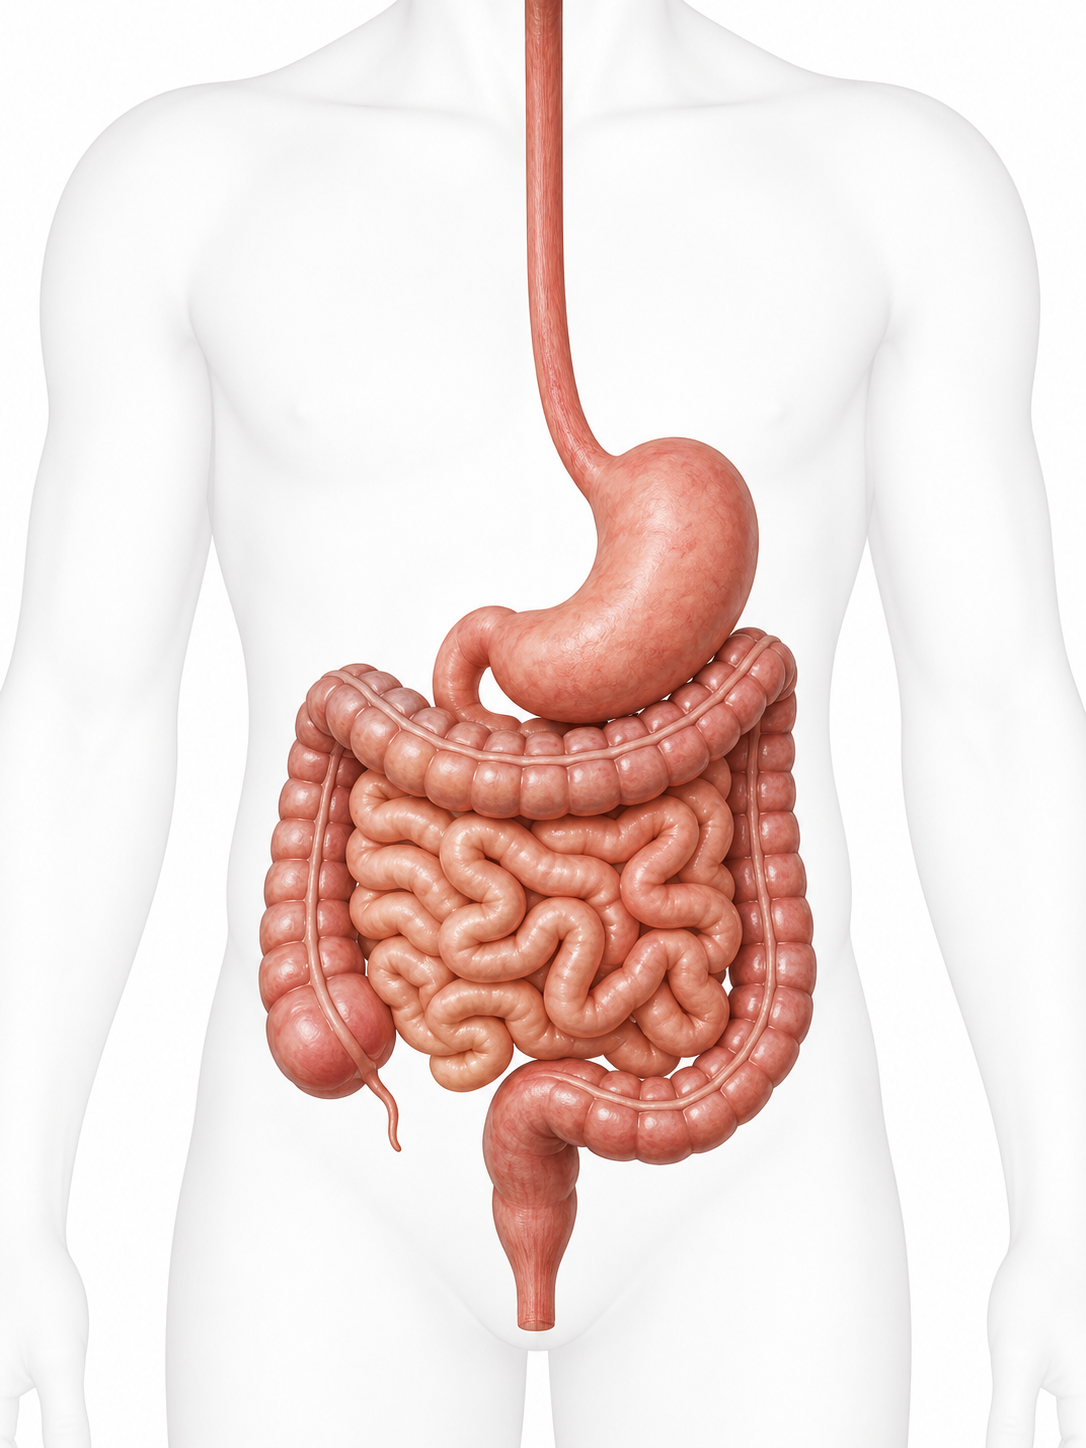
\includegraphics[width=0.5\linewidth]{images/book1/ai/fig-digestive.png}};
  \begin{scope}[x={(img.south east)}, y={(img.north west)},
      every node/.style={font=\small}]
    \draw[omDef, thick] (0.52,0.85) -- (0.72,0.88) node[right] {esophagus};
    \draw[omDef, thick] (0.66,0.62) -- (0.82,0.66) node[right] {stomach};
    \draw[omDef, thick] (0.44,0.35) -- (0.16,0.28)
      node[left, align=center] {small intestine\\ (metres, folded)};
    \draw[omDef, thick] (0.74,0.42) -- (1.04,0.40)
      node[right, align=left] {large\\ intestine};
    \draw[omDef, thick] (0.50,0.09) -- (0.66,0.05)
      node[right] {leftovers out};
  \end{scope}
\end{tikzpicture}

{\small The \omterm{def:g4:journey-of-food:tract}{digestive tract}: one tube from mouth to exit. The
\omterm{def:g4:journey-of-food:tract}{esophagus} delivers to the \omterm{def:g4:journey-of-food:tract}{stomach}; the \omterm{def:g4:journey-of-food:tract}{small intestine}'s folded
metres fill the middle, framed by the \omterm{def:g4:journey-of-food:tract}{large intestine}.}
\end{omfigure}

\begin{example}[Timing the journey]\label{ex:g4:journey-of-food:timing}
The bite of bread spends seconds in the mouth, a couple of
seconds sliding down the \omterm{def:g4:journey-of-food:tract}{esophagus}, some hours being churned
in the \omterm{def:g4:journey-of-food:tract}{stomach}, several more working through the \omterm{def:g4:journey-of-food:tract}{small
intestine}, and up to a day or more finishing in the \omterm{def:g4:journey-of-food:tract}{large
intestine}. The whole journey commonly takes one to two days.
\end{example}

\section{Digestion: from food to nutrients}

\begin{definition}[Digestion and nutrients]\label{def:g4:journey-of-food:digestion}
\emph{Digestion}\index{digestion} is the transformation of
food, along the tract, into components small and simple
enough to enter the body:
the \emph{nutrients}\index{nutrient}. Teeth and the \omterm{def:g4:journey-of-food:tract}{stomach}'s
churning break food up; \emph{digestive
juices}\index{digestive juice} --- \omterm{def:g4:journey-of-food:tract}{saliva} among them ---
dismantle it further, piece by piece, until what was bread is
a liquid mix of nutrients.
\end{definition}

\begin{example}[The bread turns sweet]\label{ex:g4:journey-of-food:sweet}
Chew a piece of plain bread very long --- a slow count of
sixty --- and a faint sweetness appears. Nothing was added:
\omterm{def:g4:journey-of-food:tract}{saliva} is already dismantling the bread into simpler, sweeter
pieces. You have tasted \omterm{def:g4:journey-of-food:digestion}{digestion} beginning.
\end{example}

\begin{proposition}[Crossing into the body]\label{prop:g4:journey-of-food:absorb}
The tract's inside is still, in a sense, outside the body ---
like the hole of a doughnut. The crossing happens in the
\emph{\omterm{def:g4:journey-of-food:tract}{small intestine}}: through its thin, deeply folded
walls, \omterm{def:g4:journey-of-food:digestion}{nutrients} pass into the \emph{blood}\index{blood},
which carries them to every part of the body
(the delivery service that \cref{ch:g4:heart-and-blood}
explores). What cannot cross --- fibres, husks --- travels
on, loses its water in the \omterm{def:g4:journey-of-food:tract}{large intestine}, and \omterm{def:g1:plants-around-us:parts}{leaves} as
droppings.
\end{proposition}
\admitted

\begin{remark}[Why the folds and the metres]\label{rem:g4:journey-of-food:surface}
Crossing takes wall surface, and the \omterm{def:g4:journey-of-food:tract}{small intestine} is built
for it: metres of length, and walls folded and refolded
inside. Stretched flat, the crossing surface would carpet a
small room --- packed into your middle. Big jobs, in the
body, get big surfaces folded small.
\end{remark}

\section{Helping digestion do its work}

\begin{method}[Digestion-friendly habits]\label{met:g4:journey-of-food:habits}
\begin{enumerate}
  \item Chew properly: the \omterm{def:g4:journey-of-food:tract}{stomach} has no teeth --- what the
        mouth skips, the \omterm{def:g4:journey-of-food:tract}{stomach} must struggle with;
  \item eat calmly, at regular mealtimes;
  \item drink water with meals;
  \item eat fibre-rich foods --- vegetables, \omterm{prop:g3:flowers-fruits-seeds:transform}{fruit}, whole
        bread: fibre keeps the leftovers moving;
  \item leave hard play or swimming for after the meal has
        settled: a hard-working \omterm{def:g4:journey-of-food:tract}{stomach} and hard-working \omterm{def:g1:my-body:parts}{legs}
        compete.
\end{enumerate}
\end{method}

\begin{example}[The stomach-ache detective]\label{ex:g4:journey-of-food:ache}
Wolfed-down lunch, then a sprint: the classic afternoon
\omterm{def:g4:journey-of-food:tract}{stomach} ache. The meal was swallowed half-chewed (rule 1
broken) and the digesting \omterm{def:g4:journey-of-food:tract}{stomach} was hurried into a race
(rule 5). The fix is not medicine but manners --- toward
one's own \omterm{def:g4:journey-of-food:tract}{digestive tract}.
\end{example}

\section{Exercises}

\begin{exercise}[$\star$]\label{exo:g4:journey-of-food:1}
Name the parts of the \omterm{def:g4:journey-of-food:tract}{digestive tract} in order, mouth to
exit.
\end{exercise}

\begin{exercise}[$\star$]\label{exo:g4:journey-of-food:2}
What happens to food in the \omterm{def:g4:journey-of-food:tract}{stomach}, and roughly how long
does it stay there?
\end{exercise}

\begin{exercise}[$\star$]\label{exo:g4:journey-of-food:3}
What is \omterm{def:g4:journey-of-food:digestion}{digestion}? What are \omterm{def:g4:journey-of-food:digestion}{nutrients}?
\end{exercise}

\begin{exercise}[$\star$]\label{exo:g4:journey-of-food:4}
In which part do \omterm{def:g4:journey-of-food:digestion}{nutrients} cross into the \omterm{prop:g4:journey-of-food:absorb}{blood}? What
happens to what cannot cross?
\end{exercise}

\begin{exercise}[$\star$]\label{exo:g4:journey-of-food:5}
Why does long-chewed bread turn faintly sweet?
\end{exercise}

\begin{exercise}[$\star$]\label{exo:g4:journey-of-food:6}
Why is the \omterm{def:g4:journey-of-food:tract}{small intestine} so long and so folded inside?
\end{exercise}

\begin{exercise}[$\star$]\label{exo:g4:journey-of-food:7}
Give three digestion-friendly habits and the reason for each.
\end{exercise}

\begin{exercise}[$\star$]\label{exo:g4:journey-of-food:8}
Try it (at table): time your next meal. How long does your
food spend in your mouth --- and how does that compare with
the days ahead of it?
\end{exercise}

\begin{exercise}[$\star\star$]\label{exo:g4:journey-of-food:9}
Diagnose \cref{ex:g4:journey-of-food:ache}'s \omterm{def:g4:journey-of-food:tract}{stomach} ache:
which two habits were broken, and what would you change
tomorrow?
\end{exercise}

\begin{exercise}[$\star\star$]\label{exo:g4:journey-of-food:10}
``Food goes into the body the moment you swallow it.''
Correct this with \cref{prop:g4:journey-of-food:absorb}:
where does food really enter the body, and what must happen
to it first?
\end{exercise}

\begin{exercise}[$\star\star\star$]\label{exo:g4:journey-of-food:11}
The cow's grass is far tougher food than your bread --- and
the cow has four \omterm{def:g4:journey-of-food:tract}{stomach} chambers, chews its food twice, and
hosts helpful \omterm{def:g1:living-or-not:living}{living things} in its gut to dismantle grass.
Using \cref{def:g4:journey-of-food:digestion} and
\cref{prop:g2:what-animals-eat:match}, explain why a
grass-eater needs this heavier machinery.
\end{exercise}
